		\section{Nombre: Piedras filosas}\label{obs.piedrasF}
	\subsection{Descripción}
	Piedras puntiagudas en forma de triángulo. Sobresalen del piso o muro de un terreno, son rígidas y no poseen ningún movimiento. Al contacto con el jugador le restan puntos de vida.
	\subsection{Esquema}
	Ver figura \ref{fig:piedrasF}.
	\begin{figure}
		\centering
		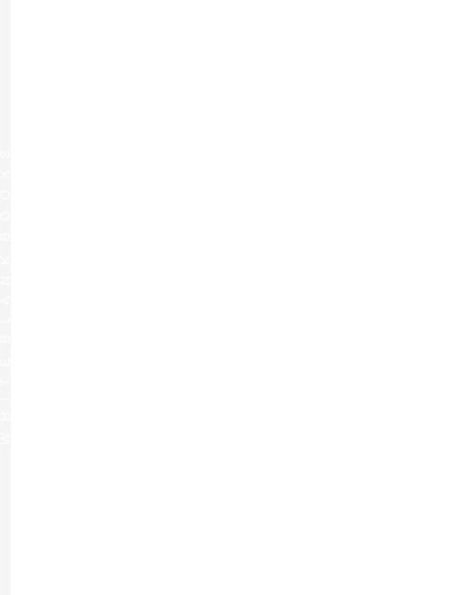
\includegraphics[height=0.2 \textheight]{Imagenes/piedrasF}
		\caption{Sacos de cacao.}
		\label{fig:piedrasF}
	\end{figure}